\chapter{Approach}
\todo{Why are we using a data-driven / machine learning approach? Show that it is complicated to do it by hand. Also write why not to do auto-tuning.}

\begin{figure}
    \centering
    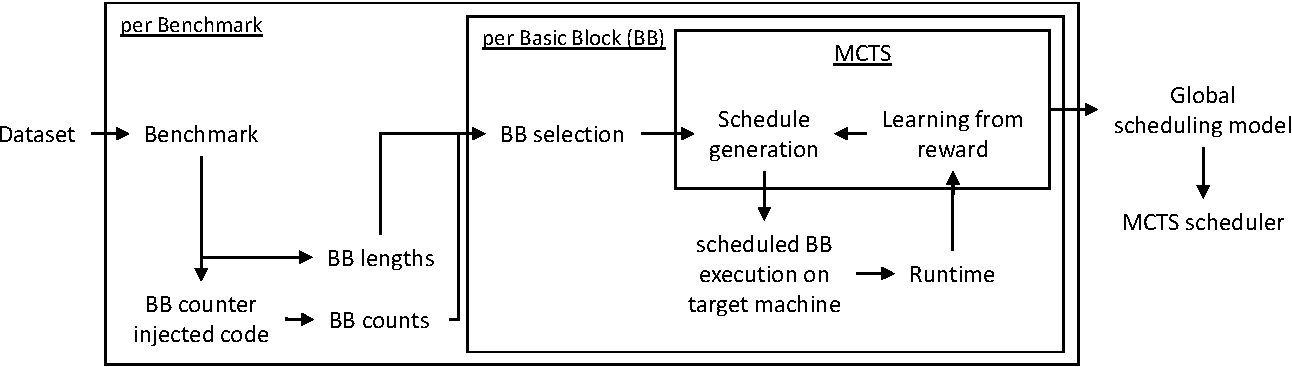
\includegraphics[width=\textwidth]{img/ppt/approach_overview-crop.pdf}
    \caption[Overview of the approach]{Overview of the overall approach. 
    The process covers the selection of basic blocks, the instruction schedule generation, the execution model, the learning process and the derivation of the final scheduler.}
    \label{fig:approach:overview}
\end{figure}
In the rest of this chapter, we present the approach used for this thesis (compare~\cref{fig:approach:overview}).
We start with an overview of the benchmark programs we used~(\cref{sec:approach:dataset}).
Then we discuss the importance of basic blocks for instruction scheduling in general and our approach specifically~(\cref{sec:approach:basicblock}).
That is followed by explaining the \ac{mcts} approach~(\cref{subsec:approach:ml:mcts}).
Eventually, we introduce our approach for combining individual \ac{mcts} models into a global model~(\cref{subsec:approach:ml:global}) and derive an applicable scheduler~(\cref{sec:approach:ml-scheduler}).

\section{Dataset}
\label{sec:approach:dataset}
For our experiments, we use benchmarks from the LLVM project~\cite{LLVM:CGO04} called LLVM Test Suite~\footnote{\url{https://llvm.org/docs/TestSuiteGuide.html}}.
The test suite contains benchmarks from the following categories
\begin{itemize}
    \item Single-Source --- built from a single C/C++ source file
    \item Multi-Source --- built from multiple C/C++ source files
    \item Micro-Benchmarks --- separate functions that are executed by google-benchmark
    \item Bitcode --- tests that are written in LLVM bitcode
    \item CTMark --- symbolic links to the other benchmarks to measure compilation performance
\end{itemize}
We select the 273 benchmarks from the Single-Source and Multi-Source categories for our experiments.
\todo{Add table?}
These categories contain benchmarks that are compiled from a single source file or multiple source files, respectively.
The benchmarks are all written in C or C++.
In addition, the test suite contains more benchmarks that are not relevant to our experiments. \todo{Why not?}

\subsection{Modified Build Process}
\label{sec:approach:build_process}
The test suite comes with Makefiles and CMake configurations to automatically build all benchmarks.
However, these are not sufficient for our approach.
We need a modified build process for all the benchmarks because we are manipulating it in several cases.
Furthermore, the compilation cannot be done by a single command because not all arguments of the separate compilation steps are available in the main compiler.
We execute the front-end, optimization, and back-end compiler phases separately to have complete control over the build process.

We have to set some compiler arguments to make the LLVM compiler front-end output LLVM \ac{ir} instead of compiling the program to an executable format.
For C programs we use \lstinline{clang}~\footnote{\url{https://clang.llvm.org/}} and for C++ programs we use \lstinline{clang++} as compilers.
However, the compiler arguments are the same.
We pass the following arguments to the front-end:
\begin{itemize}
    \item \lstinline{-O0}: to prevent optimization in this first step
    \item \lstinline{-Xclang -disable-O0-optnone}: the \lstinline{-O0} flag alone also prevents optimization in further steps, which is not what we want
    \item \lstinline{-S -emit-llvm}: to emit LLVM \ac{ir} for further processing --- instead of compiling the program completely
\end{itemize}

The LLVM optimizer \lstinline{opt}~\footnote{\url{https://llvm.org/docs/CommandGuide/opt.html}} gives a choice to select one of the predefined optimization levels or select specific optimizer runs.
When we compile a benchmark for measuring the runtime, we only use the flag \lstinline{-O3} for optimizing the LLVM \ac{ir}.
The LLVM framework makes it easy to implement new optimizer passes.
We do this to count how often a basic block is executed (see \cref{sec:approach:basicblock:selection}) and measure a function's execution time (see \cref{sec:approach:datageneration:runtime:function}).
\todo{This is not true anymore}

The LLVM back-end compiler implements two instruction schedulers before the register allocation and one after the register allocation.
The former inherit either from the C++ class \lstinline{SelectionDAG} or from \lstinline{MIScheduler}.
It depends on the target architecture which instruction scheduler will be executed by the compiler. 
It is also possible that the compiler executes both.
\todo{Maybe move this also to the bg chapter}

We manipulate the back-end by passing arguments to the LLVM static compiler \lstinline{llc}~\footnote{\url{https://llvm.org/docs/CommandGuide/llc.html}}.
This program represents the back-end phase and executes the instruction scheduling.
We use the following arguments for the back-end:
\begin{itemize}
    \item \lstinline{--pre-RA-sched=}: to select our new \lstinline{SelectionDAG} schedulers for the pre-register-allocation phase
    \item \lstinline{--misched-cutoff=0}: to disable the \lstinline{MIScheduler}
    \item \lstinline{--disable-post-ra}: to disable the post-register-allocation scheduler
\end{itemize}

We analyze the CMake configurations and extract required compiler arguments on a per benchmark level.
We categorize the extracted arguments into front-end, optimizer, and back-end phases.
Finally, we append them to the previously described arguments in the respective compilation phase.

We also analyze the test suite for execution arguments.
For example, some benchmarks read data from files or require arguments when calling them.
To execute them, we generate a shell script that calls the compiled benchmark with the required arguments.

\section{Basic Block --- Scheduling Unit}
\label{sec:approach:basicblock}
Even though there exists some research \todo{add references} on instruction scheduling on more extensive units, most compilers schedule instructions on a per basic block level.
This is also true for the LLVM compiler framework.
The advantage of this is that the limited scope avoids complicated situations and thus simplifies the scheduling problem.
For Example, do not have to deal with jump instructions.

Consequently, we also choose the basic block as the unit for instruction scheduling.
That means that we execute our experiments on individual basic blocks and learn to schedule individual basic blocks.
Later, we combine the models to generalize the knowledge.
We describe this process in detail in \cref{sec:approach:ml}.

\subsection{Selection Process}
\label{sec:approach:basicblock:selection}
Not all basic blocks provide an equal value to our experiments.
It also consumes too much time to work on all the basic blocks within the scope of this thesis (\eg compilation time, execution time, machine learning time).
Therefore, we sort our basic blocks by heuristics. 
From this list, we select as many as we need and can handle in our experiments.
We designed three heuristics which we will explain in the following paragraphs.
See \cref{tab:approach:bb_heuristics} for an example overview.

\begin{table}
    \centering
    \begin{tabular}{@{}llrrr@{}}
        \toprule
        Function & Basic Block & Length & \(\#\) Executions & Product \\
        \midrule
        kernel\_floyd\_warshall\_StrictFP & for.body6 & 23 & 536,870,912 & 12,348,030,976 \\
        kernel\_floyd\_warshall & for.body6 & 23 & 536,870,912 & 12,348,030,976 \\
        print\_element & entry & 25 & 1,048,576 & 26,214,400 \\
        kernel\_floyd\_warshall\_StrictFP & for.cond4.preheader & 17 & 1,048,576 & 17,825,792 \\
        \(\cdots\) & \(\cdots\) & \(\cdots\) & \(\cdots\) & \(\cdots\) \\
        xmalloc & entry & 8 & 2 & 16 \\
        main & entry & 11 & 1 & 11 \\
        \bottomrule
    \end{tabular}
    \caption[Basic block heuristics for the floyd-warshall benchmark]
    {
        The tables shows an excerpt of the basic block heuristics (see \cref{sec:approach:basicblock:selection}) for the floyd-warshall benchmark. 
        The basic blocks are sorted by the last heuristic, which is the product of the length and execution count. 
        From this list the table shows the top four and last two basic blocks in the benchmark.
    }
    \label{tab:approach:bb_heuristics}
\end{table}

\subsubsection{Longest Basic Blocks}
\todo{Add note about influence of pipeline length}
\todo{More different instructions use more functional units of the processor}
The number of instructions in a basic block correlates with the number of possible schedules.
Consequently, we can learn more from a basic block when there are more different scheduling situations available.
For example, we will see more scheduling situations in a basic block containing 20 instructions than in a basic block containing only three instructions.

We implemented a hook into the LLVM framework to count the number of instructions in a basic block.
This hook prints the number of instructions in each basic block during the compilation process.
From this output, we put together a list with all basic blocks and their lengths (see \cref{tab:approach:bb_heuristics}).

\subsubsection{Most Executed Basic Blocks}
Some basic blocks are significantly more often executed than others.
For example, basic blocks in the bodies of loops run often.
A basic block in the error checking code of the beginning of a program might only execute once.
Often executed basic blocks influence the overall runtime a lot.
Hence, we are more interested in optimizing these.
See \cref{tab:approach:bb_heuristics} for an example.

We implemented a LLVM optimizer pass for injecting counters into a program.
Optimizer passes take LLVM \ac{ir} files as input and output the code in the same file format.
Our pass injects one global 64 bit counter variable for each basic block into the code.
Next, the pass adds instructions into the beginning of each basic block, which increase the corresponding counter by one.
At the end of the main function the pass adds a format string and injects a call to the \lstinline{printf} function to print all the counter values and corresponding basic block names.

The optimizer pass must be compiled with the LLVM framework.
We include the optimizer pass into our build process (see \cref{sec:approach:build_process}).
There, we add a call to the LLVM optimizer \lstinline{opt} with the argument \mbox{\lstinline{-passes=dyn-bb-count}}.
To actually get the counts, we build a benchmark with this optimizer pass and and execute it.
The benchmark will then print the counter values.

\subsubsection{Most Executed and Longest Basic Blocks}
\todo{Include discussion about variance in resulting basic blocks}
\todo{most influence on overall runtime}
The previous two heuristics are helpful on their own, but we are most interested in basic blocks that combine the two aspects.
For example, the most executed basic block can still come from a very simple loop with few instructions in the loop body.
We compute the product of the two heuristics to get a combined heuristic.

\section{Learning to Schedule}
\label{sec:approach:ml}
\subsection{Local MCTS Model}
\label{subsec:approach:ml:mcts}
\todo{Explain why we use max instead of avg. See \eg transition from data/mcts-max-vs-avg/svg/8752639012199.svg to data/mcts-max-vs-avg/svg/8749356177210.svg LoopRestructuring-dbl,s2233,for.body20}
\subsection{Global Model}
\label{subsec:approach:ml:global}
\subsubsection{Look Up Model}
\subsubsection{Support Vector Machine Model}
\subsubsection{Neural Network Model}

\section{Data Generation}
\tobechecked
We cannot build our data-driven models (see \cref{sec:approach:ml}) directly from our dataset, described in \cref{sec:approach:dataset}.
Learning from this dataset requires some transformation from the code to a metric we are interested in.
Many metrics can be chosen for optimization \eg runtime, energy consumption, cache misses, processor stalls.
We focus on optimizing the instruction scheduling for short runtimes.
To generate data for our MCTS approach we need a mapping from instruction schedules to runtimes.

The most reliable approach is to measure the runtime while executing the code.
\todo{Discuss these in related work. Check Ithemal paper for more ressources}
However, research on approaches that rely on analytical models exists~\cite{llvm:mca, mendis2019ithemal, taha2003instruction, laukemann2018automated}.
We will choose the classical approach of runtime measurements, since we have access to the hardware and the resulting data will be more accurate.
Therefore, we compile the code with varying instruction schedules and execute it to measure its runtime.
We discuss various aspects of this in the remainder of this section.

\begin{figure}
    \centering
    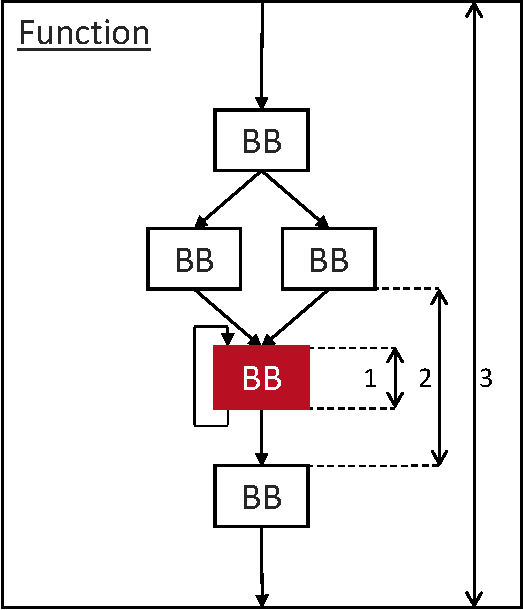
\includegraphics[scale=0.8]{img/ppt/runtime_measurement_scopes-crop.pdf}
    \caption[Possibile scopes for measuring runtimes]{The outer box represents a function. 
    The function consists of multiple basic blocks (BB) where different possible branches are caused by if/else statements and loops. 
    The diagram shows three possible runtime measuring scopes to measure the runtime of the filled basic block.
    Method 1 shows a measuring inside of a basic block. 
    With method 2, the measurement starts with the end of the last basic block and ends with the start of the next one.
    Method 3 measures the complete function which surrounds the basic block.}
    \label{fig:approach:runtime_scopes}
\end{figure}

\subsection{Runtime Measurement Unit}
\tobechecked
The metric we are interested in specifically, is the relative runtime compared to a baseline runtime.
Runtime overheads can be ignored in our approach, as long as they are constant over multiple runs.
Thus, various possibilities for placing the start and stop events of the timer exist to accomplish runtime measurements of fractions of the applications code.
The objective is to minimize noise and get reliable, reproducable measurements.
We discuss the possibilities of making measurements on basic block, function and application scope and relevant aspects to these possibilities.

\subsubsection{Application}
\tobechecked
\label{sec:approach:datageneration:runtime:app}
The most straight forward approach to measuring the runtime of a piece of code is to measure the runtime of its whole application.
The disadvantage is, that we include many more instructions in the measurement than we are interested in.
This generates lots of noise from various possible sources (\eg from \ac{io} instructions like opening files, printing to the screen or varying latencies for memory accesses).
Also, the longer the runtime of a program, the higher is the probablity that the operating system will interrupt the execution for more important processes.
Depending on the used measurement method (see \cref{sec:approach:datageneration:runtime_methods}), this will be included or not be included in the measurement.
These disadvantages make this approach unreliable and not usable for us because we are interested in the short runtime of a single basic block.

\subsubsection{Function}
\tobechecked
\label{sec:approach:datageneration:runtime:function}
A finer grained approach is to start the timer at the beginning of the function or method that contains the basic block of interest and stop the timer at the end of the function (see method 3 in \cref{fig:approach:runtime_scopes}).
There come several problems with this approach.

Compared to measuring the runtime of the whole application (see \cref{sec:approach:datageneration:runtime:app}) this approach executes only a small fraction of the code.
This results in a lower probablity for variances in the measured runtimes due to less \ac{os} interrupts, less memory and \ac{io} accesses.
Thus, the precision of these measurements is higher.

Notice in \cref{fig:approach:runtime_scopes} that there are different control paths are possible in a function, based on if/else statements or loops.
This can be problematic in a general setup.
However, the benchmarks we use and the data we insert to them are deterministic, \ie the same paths are taken with each benchmark execution.
Theoretically, if there were no variance in the measurements, the shortest measured execution time would always correspond to the same execution path.
In practice, we get many varying measurements because of different execution paths.
That makes it difficult to differentiate between execution paths and variance in the measurements.

\subsubsection{Basic Block}
\tobechecked
The most intuitive approach is to measure only the runtime of the basic block we are interested in.
We eliminate all extra processor instructions that we are not interested in.
However, we can still get runtime variations for different reasons:
\begin{itemize}
    \item The basic block could call other functions which could execute varying branches. 
          See \cref{sec:approach:bbisolation} for a discussion about this.
    \item The \ac{os} could interrupt the execution. 
          But the probablity decreases with shorter code fragments.
\end{itemize}

One requirement can not be met in all situations is that we require a very precise timer.
These timers usually depend on the hardware directly, \ie the hardware must provide such functionality to measure runtimes.
This is possible on our chosen hardware and is discussed in more detail in \cref{sec:approach:hwpercounter}.

Thus, as this is a feasible solution for our experiments we have chosen to measure the runtime of basic blocks alone.
    
\subsection{Runtime Measurement Methods}
\label{sec:approach:datageneration:runtime_methods}
\todo{Could add little experiment where we compare hardware timers vs OS access}
\subsubsection{Profiling}
\begin{itemize}
    \item What: Profilers are a bad choice for measuring precise runtimes
    \item Why: They are just not designed for it, they serve other purposes.
        Profilers are making snapshots of the running system to measure performance. 
        There is no measurement from point A to point B which leads to inaccuracies
    \item How: Read e.g. the paper of gperf \cite{graham1982gprof}
\end{itemize}
\subsubsection{Operating System Methods}
% In linux(C): clock_gettime().
% Windows: QueryPerformanceCounter().
% C++: std::high_resolution_clock().
These might return different clocks depending on the used hardware.
Returns the time from the hardware the OS runs on.
Has overhead but also handles problems.
Typically best for measurements in microseconds range and longer.
Include pinning processes to cores and isolating cores.
\subsubsection{Hardware Performance Counters}
\label{sec:approach:hwpercounter}
Accessed by assembly instructions.
% x86: 'rdtsc' Saves current value into EDX:EAX registers
% ARM32: mrc p15m, 0, \%0, c15, c12, 1
% AARCH64: mrs \%0, PMCCNTR_EL0
% Aurora: fencei; smir \%0, \%usrcc
Measurements in CPU cycles.
Lowest overhead available.
Access might be protected (Linux module required).

\subsection{Execution Unit}
\todo{Provide runtime example data}
\label{sec:approach:exec_unit}
For the learning process, we have to execute the differently scheduled basic blocks many times.
This can be time intensive, and many lines of code are executed that we are not interested in.
The scope of the thesis forces us to extract the basic block from the benchmark and execute it in isolation.
Here, we discuss the advantages and disadvantages of the two possible approaches.

\subsubsection{Benchmark}
The first option is to execute the complete benchmark for every new schedule that was generated during the learning process.
The advantage is, that we execute the original basic block like it would appear in the real benchmark.
The problem with this approach is that the execution time of a benchmark can be high and makes the execution the bottleneck in our pipeline.
Many benchmarks in our dataset take several minutes to execute on a RaspberryPi 3B.
So, executing always the whole benchmark is costly to even get only one runtime measurement per schedule.
In order to get statistically relevant runtimes, we have to measure them multiple times because.

\subsubsection{Basic Block}
The alternative to executing the whole benchmark is to extract the scheduled basic block from the benchmark and execute in isolation.
By using this approach we reduce the execution time to a minimum and do not execute code we are not interested in.
Consequently, we can execute the benchmark many times and get statistically reliable runtime measurements.
The disadvantage is that we have to slightly modify the basic block or the program will crash.

\subsection{Basic Block Isolation}
\label{sec:approach:bbisolation}
As discussed in \cref{sec:approach:exec_unit}, we are forced to execute basic blocks isolated from the benchmark.
To make a basic block executable we isolate it and insert it as inline assembly into our minimal C++ framework.

\subsubsection{Basic Block Extraction}
\todo{include numbers on speedup vs. benchmarking full function}
First, we compile the benchmark and schedule the basic block with our modified compilation process (see \cref{sec:approach:build_process}) into assembly files.
Next, we extract the basic block instructions from the assembly file.
Then, we modify the basic block instructions slightly to prevent execution and compilation errors and as a last step we inject it into our C++ framework.

The assembly code can contain some lines that will make our framwork crash.
We are forced to modify or delete these lines.

Assembly files contain comments, labels and assembler directives which will be removed.
Comments are useless lines for the execution task. 
The labels are not required, as we will not jump to other instructions.
And assembler directives represent commands to the assembler program for bookkeeping, storage reservation and other purposes.
These could interfere with our compilation process and are also removed.

Basic blocks can contain jump instructions as the last instruction and function calls in any position.
We only schedule the instructions in the given basic block, so we are also only interested in its own runtime.
Executing other code, which could internally chosse different paths would add noise to our measurements.
To prevent this uncontrolled program execution, we simply remove jump and call instructions.
The removal of these instructions might slightly reduce the execution time, but the reduction is constant over all executions with different schedules.

In order to prevent segmentation faults, we have to redirect all memory accesses to a memory area that we are allowed to read and write to.
This affects all load and store instructions.
In our framwork we allocate 8 byte on the stack where we redirect all memory accesses to.
This means also that all memory accesses are cache hits and we have a controlled environment in this aspect.

\todo{Show example}

\subsubsection{Isolated Basic Block Execution}
From extracted basic block create inline assembly with stack variable. Now executable from C/C++.
Warmup 100 runs. Timings 1000 runs. 
\subsection{Computing Rewards From Runtimes}
There are some outliers in the runtimes. Sort runtimes, cutoff lower and upper 5\% of the runtimes to remove outliers and compute avg of the rest.
What could be reasons for outliers?
Show some distributions of measurements to justify why we are throwing away data.

\section{Application of the Learned Model}
\label{sec:approach:ml-scheduler}

% Probably wrong place here, but compare approach with auto-tuning approach.
% Why not use auto-tuning? Search space size, and lack of generalization could be a reason

% \section{Breaking down the problem (maybe just chapter introduction)}
% \begin{itemize}
%     \item Schedulers run on basic blocks -> Select the most executed (hottest) BB's
% \end{itemize}

% \section{Experimentation Pipeline}
% Explain and illustrate the pipeline incl. injection of timers and counters

% \section{Benchmarking}
% \begin{itemize}
%     \item Benchmarking methods: Instrumentation, sampling -> only instrumentation makes sense here. Justify this with instrumentation vs. sampling results (our timing vs. perf timing)
%     \item Where to inject timer in BB DAG
%     \begin{itemize}
%         \item We only want to measure optimized code, but not too kleinteilig because of lacking accuracy. Problematic code is IO code
%         \item Time whole function?
%         \item Time only relevant BB's with surrounding ones (e.g., loop headers) -> Where exactly place the the timer
%         \item Provide data and examples to demonstrate decision making
%     \end{itemize} 
% \end{itemize}
% \subsection{Implementation}
% Injection of the \lstinline[language=C++]{std::chrono::high_resolution_clock}

% \section{Training setup}
% Compile with default scheduler and measure its runtime.
% Compile with our scheduler, execute the program, measure the runtime and use it to train the agent.

% \section{MCTS}
% \subsection{Tree Modeling}
% We probably want to model the interdependence between instructions. 
% But depending on the benchmark programs, only a small fraction of possible edges between instructions are available.

% \eg When in the benchmark a MOV was scheduled and after that, there are only SUB and ADD.
% We cannot schedule another MOV even though that might be the optimal schedule.

% This problem must be addressed somehow.
% There are different possibilities:
% \begin{itemize}
%     \item Declare all the states with their possible successors to different states.
%     The problem with this approach is that the number of states gets very high and most states are visited rarely, possibly only in the given benchmark/basic-block.
%     \item Probablistic Policy like in RL. (Does that exist for MCTS?)
%     This might solve the problem with unavailable edges, but it does not help with learning at all because the agent would have to learn which instructions are available, too.
%     Which is not what we want.
% \end{itemize}